\documentclass[10pt]{article}

\usepackage[mode=buildnew,subpreambles=true]{standalone}
\input{preamble}

\title{\bf Error in the cloning algorithm}
\author{Yann-Edwin Keta}
\date{January 5th, 2019}

\begin{document}

\maketitle

We consider the following modified equation of rotational motion,
\begin{equation}
\dot{\theta}_i = - g \, N \, \frac{\partial}{\partial \theta_i} |\underline{\nu}(t)|^2 + \sqrt{\frac{2}{\alpha \, \text{Pe}}} \xi_i,
\end{equation}
with $g$ a free parameter.\\

According to notes by Takahiro, summarised in \href{https://yketa.github.io/DAMTP_2019_Wiki/#ABP%20cloning%20algorithm}{this tiddler}, we should have that
\begin{equation}
\left. s \, w_{\text{mod}}(0, \tau) \right|_{s=0} =  \frac{1}{N} - \underbrace{\frac{1}{\tau} \int_0^{\tau} |\underline{\nu}(t)|^2 \, \text{d}t}_{\mathcal{I}_1(0, \tau)} - g^2 \, \alpha \, \text{Pe} \, \underbrace{\frac{1}{N \, \tau} \int_0^{\tau} |\underline{\nu}(t)|^2 \, \sum_{i=1}^N \sin^2(\theta_i(t) - \varphi(t)) \, \text{d}t}_{\mathcal{I}_2(0, \tau)},
\label{swmod}
\end{equation}
with
\begin{equation}
\lim_{\tau \rightarrow \infty} \mathcal{I}_1(0, \tau) = \left<|\underline{\nu}(t)|^2\right>_{\text{mod}} = \frac{1}{N}\frac{1}{1 + g \, \alpha \, \text{Pe}},
\label{I1}
\end{equation}
which we check in figure \ref{testI1}.

\begin{figure}[H]
\centering
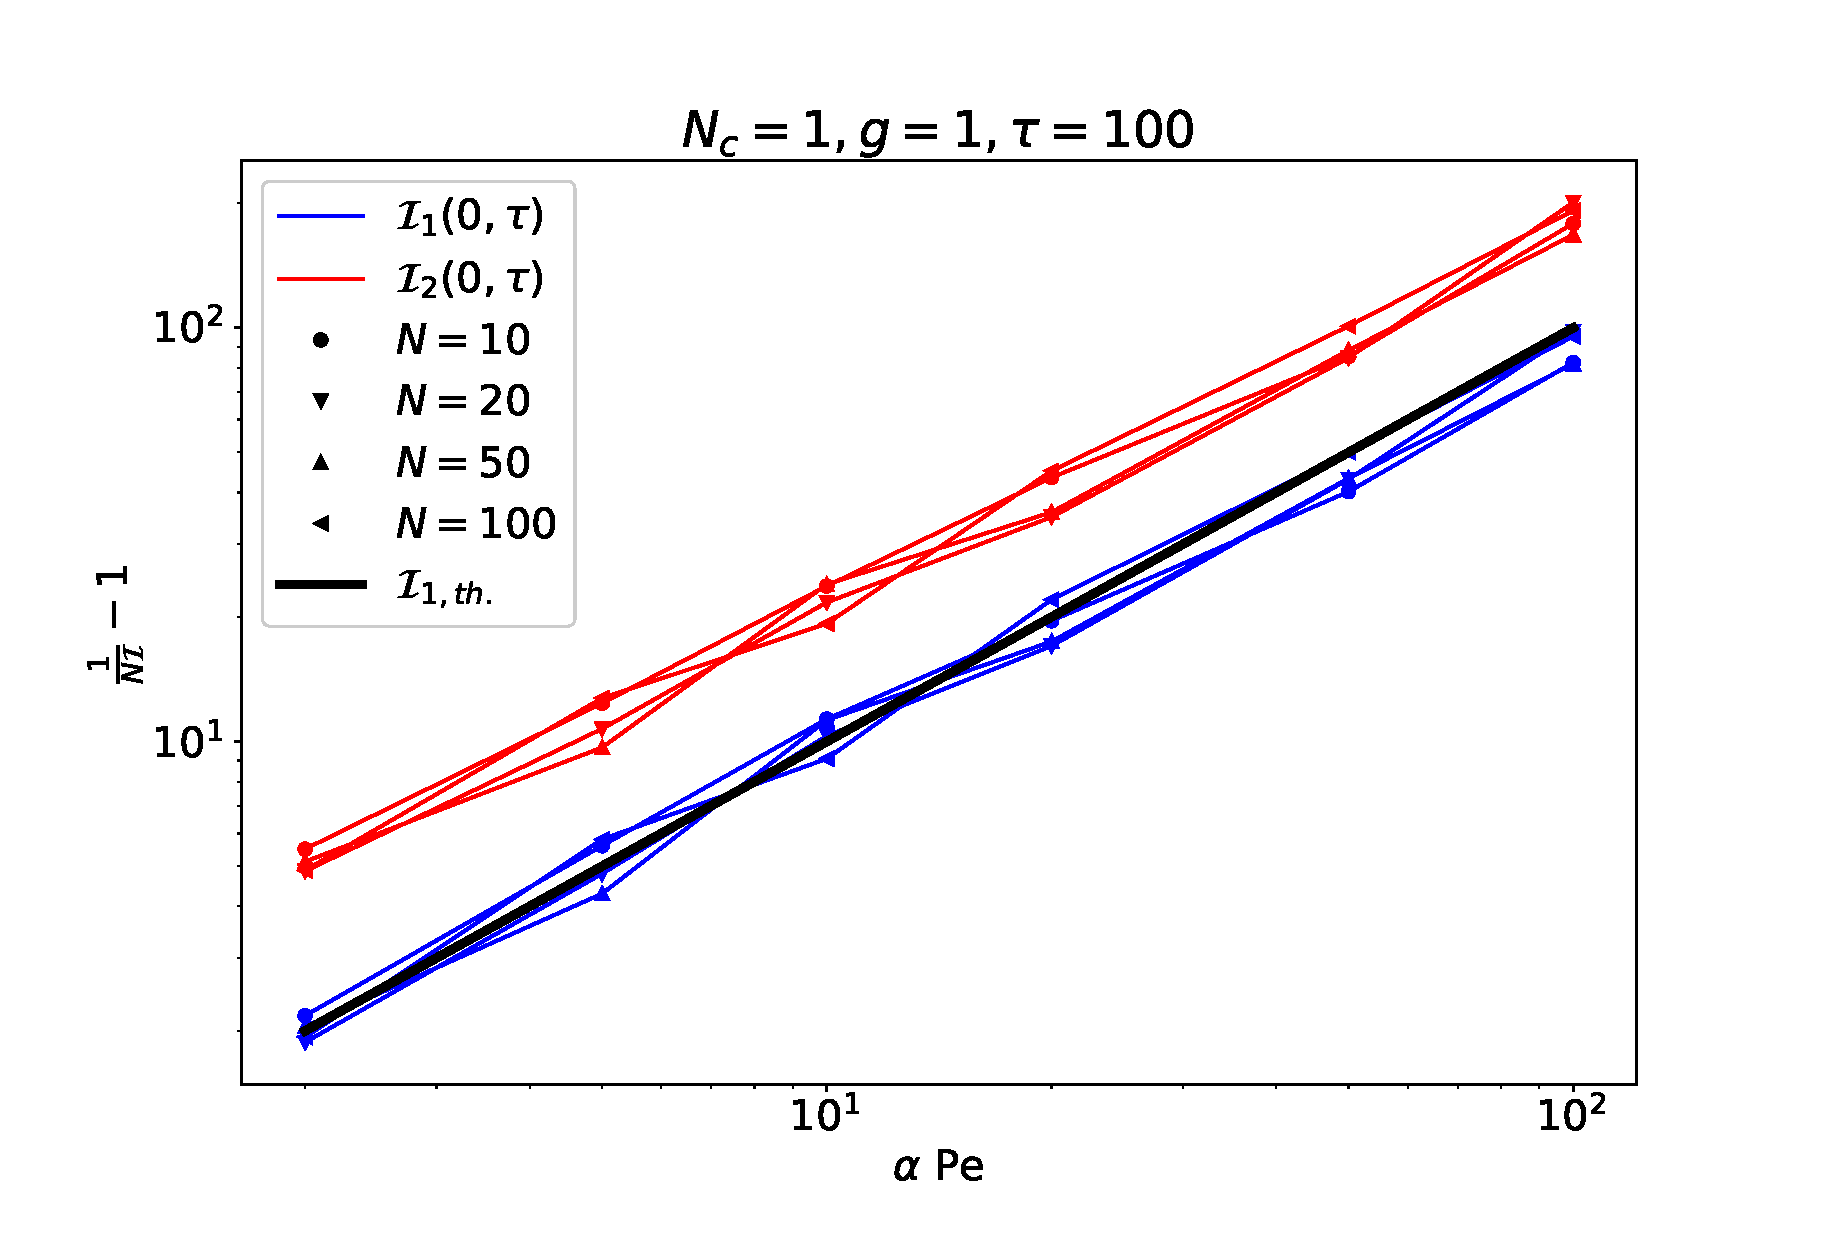
\includegraphics[width=0.65\textwidth]{testI1.eps}
\caption{Output from our cloning algorithm.}
\label{testI1}
\end{figure}

Considering a single clone, $N_c = 1$, we approximate the scaled cumulant generating function with
\begin{equation}
\psi(s=0, \tau) = \left. - s \, w_{\text{mod}}(0, \tau)\right|_{s=0},
\end{equation}
and we note that
\begin{equation}
\psi(s=0, \tau) = \left.\frac{1}{N \, \tau} \log\left<e^{-s \, N \, \tau \, w(0, \tau)}\right>_0\right|_{s=0} = 0,
\end{equation}
which with equations \ref{swmod} and \ref{I1} should lead to
\begin{equation}
\left. \mathcal{I}_2(0, \tau) \right|_{s=0} = \frac{1}{N} \frac{1}{g + g^2 \, \alpha \, \text{Pe}},
\end{equation}
and in particular, for $g = 1$, to
\begin{equation}
\left. \mathcal{I}_2(0, \tau) \right|_{s=0, g=1} = \left. \mathcal{I}_1(0, \tau) \right|_{s=0, g=1},
\end{equation}
which we see from figure \ref{testI1} is not satisfied.\\

We can see this discrepancy from the fact that
\begin{equation}
0 \leq \frac{1}{N} \sum_{i=1}^N \sin^2(\theta_i(t) - \varphi(t)) \leq 1,
\end{equation}
and thus
\begin{equation}
\mathcal{I}_2(0, \tau) \leq \mathcal{I}_1(0, \tau).
\end{equation}
Moreover, we have that the unbiased dynamics, $s = 0$, should not display orientational order, $|\underline{\nu}(t)| \approx 0$ for $N \rightarrow \infty$. Heuristically, considering that the $\theta_i$ are randomly distributed, we should get that
\begin{equation}
\left<\frac{1}{N} \sum_{i=1}^N \sin^2(\theta_i(t) - \varphi(t)) \right> \approx \left<\sin^2\right> = \frac{1}{2},
\end{equation}
which may explain the approximate relation
\begin{equation}
\mathcal{I}_2(0, \tau) \approx \frac{1}{2} \mathcal{I}_1(0, \tau),
\end{equation}
we observe numerically.

\end{document}
